

\begin{center}
\begin{figure*}
\begin{tabular}{c}
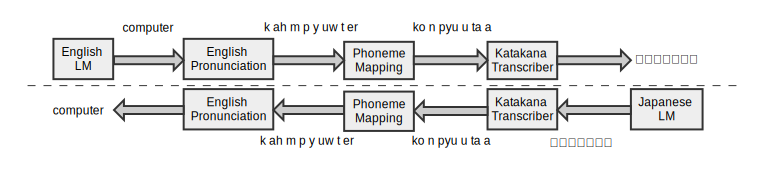
\includegraphics[scale=0.58]{figures/fsts}\tabularnewline
\end{tabular}\caption{\label{font-table} The transliteration generative story as a cascade of FSTs . \textbf{Top:} transliteration of the word ``computer'' to Japanese. \textbf{Bottom:} the reverse process. Each box represents a transducer. In PAT for deciphering transliterations, the two cascades are jointly trained to maximize both the data log-likelihood and the parameter agreement of the two (shaded) phoneme mapping models.}
\label{fig:fsts}
\end{figure*}
\end{center}

In the following two sections we show that PAT leads to better transliteration models even without parallel data. We first briefly describe a generative model for transliterated terms, due to Knight and Graehl, and subsequently report the results of a carefully designed decipherment experiment.

\subsection{Transliterations}

Transliteration is a mapping of terms between writing systems of different languages. 
Usually, the transliterator tries to preserve the sound of a term as it is spoken in the original language. For example, the word ``computer'' in Japanese is transliterated to Japanese as ``ko n pyu u ta a'' (in Romaji). 
The \emph{back-transliteration} task asks to reverse this process by restoring transliterated foreign words to their original script.

Knight and Graehl \cite{KG98} model the transliteration of an English
term $w$ into a Japanese $k$ using a generative story, encoded as
a cascade of four finite state transducers (see top of Figure \ref{fig:fsts}): 
\begin{enumerate}
\item First, a word $w$ is generated according to an English language model
$\PP(w)$
\item $w$ is then mapped to a sequence of English
phonemes $e=(e_{1},\ldots,e_{M})$ according to a pronunciation model
\item Each phoneme $e_{m}\in e$ is mapped to a sequence of Japanese phonemes
$j_{m}$ according to a phoneme mapping model $\PP(j_{m}|e_{m})$
in practice, restricted to 1-to-1 or 1-to-2 phoneme mappings.
\item Finally, the entire Japanese pronunciation sequence is mapped to a
Japanese word $k$ in Katakana script
\end{enumerate}
Knight and Graehl (\cite{KG98}) construct and train these FSTs independently.

In particular, to train the phoneme mapping model $\PP(j_{m}\mid e_{m})$ a parallel
phoneme corpus $\{(e_{n},\, j_{n})\}$ is prepared and its likelihood is then maximized using EM. 

\subsection{Deciphering Transliterations}
Collecting parallel data is often a time consuming and laborious process.
To combat the need for parallel data Ravi and Knight \cite{RK09} suggest learning to transliterate in the \emph{decipherment} setting (for simplicity, they assume a single pronunciation per term):
In decipherment, only Japanese pronunciations $J=\{j_{n}\}_{n=1..|J|}$ need be collected.
Treating the English pronunciation as missing data, a phoneme sequence $j$ is viewed as being generated by all English pronunciations $e$ via the marginalization equation $$P(j) = \sum_{e}\PP(e)\cdot \PP(j\mid e)$$
and the data log-likelihood takes the form:
\begin{align}
L(J)& = \sum_{j\in J} log \sum_{e} \PP(j\mid e)\cdot \PP(e)
\end{align}
where the summation ranges over all English words $w$ in the language model with. pronunciation $e$.

%We note a few points:
%\begin{itemize}
%\item The computational cost of solving this problem is much higher than the parallel case since we are forced to use the language and pronunciation models during training time. 
%\item Only the phoneme mapping parameters $P(j_{m}\mid e_{m})$ are trained while
%the other FSTs' parameters are kept fixed.
%\end{itemize}

\subsection{Parameter Agreement Training}
To apply PAT, we reverse the generative story as follows: First, a word $k$ is sampled from a Japanese language model (estimated over Katakana only), it is then processed using the inverse FSTs, in the reverse order (As illustrated at the bottom of Figure \ref{fig:fsts}))
Independent training in the reverse direction amounts to collecting an additional (monolingual) English corpus $E=\{e_n\}_{n=1..|E|}$ and then maximizing its log-likelihood:
\begin{align}
L(E)& = \sum_{e\in E} log \sum_{j} \QQ(e\mid j)\cdot \QQ(j)
\end{align}
In PAT, we maximize the joint regularized objective function:
\begin{align}
L(J) + L(E) + \lambda R(\PP(j|e), \QQ(e|j))
\label{eqn:dec_obj}
\end{align}

%Overall, less than 200 parameters have value larger than 0.01 in the parallel case, while
%in decipherment, the number orders on 400. As expected, ordinary EM
%leaves a lot of room for ambiguity in the decipherment case.

\begin{center}
\begin{figure*}(t)
\begin{tabular}{ccc}
 &  & \tabularnewline
 & 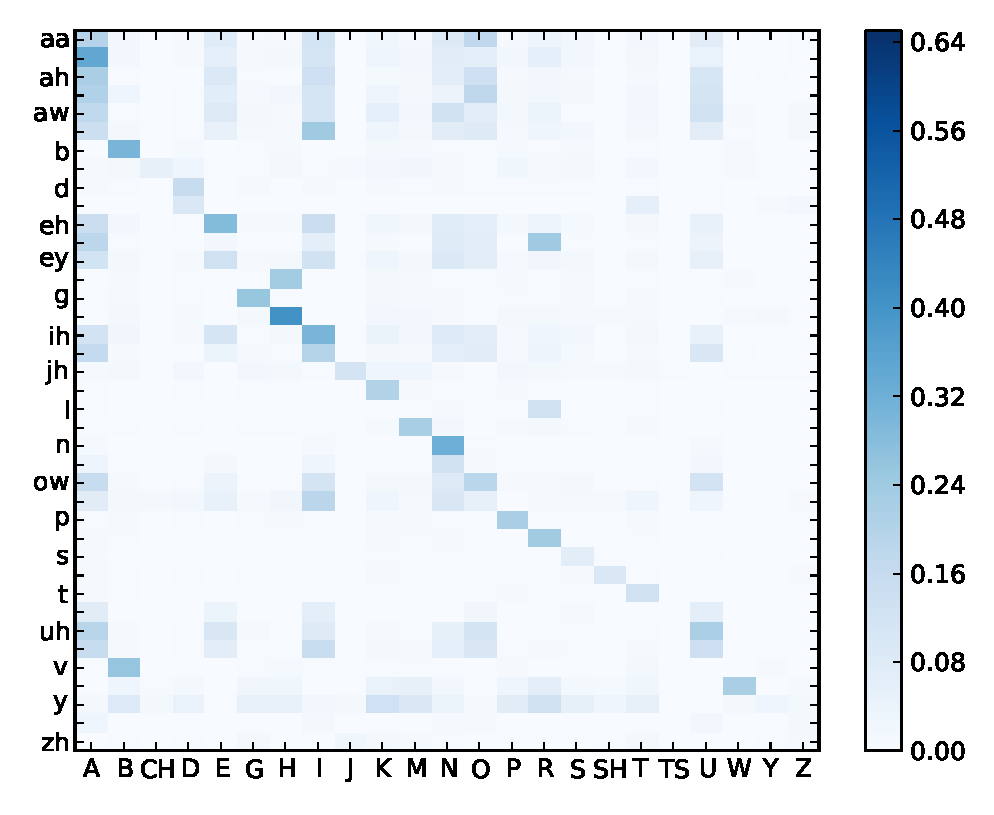
\includegraphics[scale=0.4]{figures/model_11_vanilla} & \includegraphics[scale=0.4]{figures/model_11_gm}\tabularnewline
 &  & \tabularnewline
\end{tabular}
\caption{\label{font-table} The 1-to-1 phoneme mapping submatrix of the model learned by ordinary EM (left) and parameter agreement with the geometric mean regularizer. Parameter agreement produces sparser models.}
\end{figure*}
\end{center}

\subsection{Decipherment Experiments}
Ravi and Knight (\cite{RK09}) compare back-transliteration whole-name error rates (WNER) on
a list of 100 US senator names (In WNER, a decoding is correct if both the first and last name are decoded correctly).
They report 40\% error rate in the
parallel setting, and a 73\% error rate when using their best decipherment setting.

In order to compare PAT against independent training, we produced similar decipherment setting as in \cite{RK09}.
For the FST machinery, we prepared:
\begin{itemize}
\item English and Japanese pronunciation FSTs. The English pronunciation FST was constructed according to the CMU pronunciation dictionary. A Japanese pronunciation FST was hand built.
\item Pronounceable English word unigram LM constructed over the top ~40K most frequent capitalized words in the gigaword corpus.
\item Pronounceable Japanese word unigram LM constructed over the top ~25K most frequent Katakana terms in the Japanese news 2005-2008 Leipzig corpora (http://corpora.informatik.uni-leipzig.de/download.html)
\item We designed and initialized the phoneme mapping FSTs according to the best setting reported in \ref{RK09} (e.g., consonant parity. See details in the paper.)
\end{itemize}
For training data we took $E$ and $J$ to be all pronunciations from the two language model.
It is important to note that these $E$ and $J$ are far from being parallel, since they were collected over disjoint corpora.

In training time we maximized the objective (Equation \ref{eqn:dec_obj}) with respect to the phoneme mapping models $\PP(e\mid j), \QQ(j\mid e)$ with  $\lambda\in\{1,2,3,4\}$. Training was stopped after 15 EM iterations.

We used a development set to select the best iteration, $\lambda$ and stretch factor $\alpha \in \{1,2,3\}$. The development set consistent of 50 frequent Japanese words according to the Japanese LM and their English origin.

We compiled our own list of 100 US statesmen and used it as a test set.




\begin{itemize}
\item no Parallel Data
\item Fair Experiment setting

\begin{itemize}
\item Data Collection, Numbers
\item Generate the entire LM both ways.
\item Comparison of results and sparsity, image for sparsity
\end{itemize}
\end{itemize}